\documentclass[a4paper,11pt,twocolumn]{jarticle}
\usepackage[dvipdfmx]{graphicx}
\usepackage{evocomp}
\usepackage{fancyhdr}
\usepackage{amsmath,amssymb}
\usepackage{bm}
\usepackage{ascmac}
\usepackage{mathtools}
\usepackage{comment}
\usepackage{subfigure}
\usepackage{algorithm}
\usepackage{algpseudocode}
\usepackage{setspace}
\usepackage{multirow}
\usepackage{lscape}
\usepackage{fullpage}
\usepackage{ulem}
\usepackage{longtable}
\usepackage{multicol}


\pagestyle{empty}

\renewcommand{\headrulewidth}{0.0pt}
\renewcommand{\footrulewidth}{0.0pt}
\renewcommand{\Return}[1]{\State \textbf{return} #1}

\begin{document}
\twocolumn[%
\begin{center}

%---------------------------------------------------------------------------
% ヘッダ
%---------------------------------------------------------------------------
\beginheader


%---------------------------------------------------------------------------
% 発表題目    書式:\title{日本語タイトル}{日本語サブタイトル} 「\\」で改行できます
%---------------------------------------------------------------------------
\jtitle%
{グラフ構造によるアルゴリズムの表現を用いた AutoML-Zero の提案}

%---------------------------------------------------------------------------
% 著者名      書式:\author{日本語著者名}{英語著者名}
%---------------------------------------------------------------------------

\begin{authors}
%%%%
%\name{所属番号(下記の\affに対応)}{著者名を記入},
%%%%
\name{1}{三嶋 隆史},
\name{1}{小野 功},
%%%%
\end{authors}



\begin{affiliation}
\aff{1}{東京科学大学情報理工学院},
\end{affiliation}

%---------------------------------------------------------------------------


\endheader
%--------------------------------------------------------------
\end{center}
]%

%--------------------------------------------------------------
% 英文タイトル
%--------------------------------------------------------------

\etitle{Proposal of AutoML-Zero Using Graph-Based Algorithm Representation}

%--------------------------------------------------------------
% 英語語著者名
%--------------------------------------------------------------
% ename{1}{***} : 所属1の氏名
% ename{2}{***} : 所属2の氏名 のようにする.

\ename{1}{Ryuji Mishima (mishima.r.ab@m.titech.ac.jp)}
\ename{1}{Isao Ono (isao@dis.titech.ac.jp)}


%--------------------------------------------------------------
% 英語所属
%--------------------------------------------------------------
% eaff{1}{***} : 所属1
% eaff{2}{***} : 所属2 のようにする.所属の引数は4まで.
% ※日本語の所属と対応させること.


\eaff{1}{%
School of Computing, %
Institute of Science Tokyo%
}


\vspace{3mm}

\kanjiskip=.1zw plus 3pt minus 3pt
\xkanjiskip=.1zw plus 3pt minus 3pt
%---------------------------------------------------------------------------
% 本文
%---------------------------------------------------------------------------

\section{はじめに}\label{sec:intro}

AutoMLは, 機械学習のモデルを自動で最適化する手法として注目されてきた. これまでのAutoMLに関する研究の多くは, 計算コストを抑えるために人間のデザインに大きく依存した制約付きの空間を探索している. 例えば, ニューラルネットワークの構造探索では, 事前に専門家が用意した経験則的に性能が高くなる層を構成要素として使うことで, 最適化の対象を構成要素の組合わせやハイパーパラメータに限定したり, 重みの更新方法として常に誤差逆伝搬法を用いることで探索空間を制限している\cite{Zoph_2016}\cite{Real_2019}\cite{Tan_2019}.

一方で, Estebanらが言及しているように, 探索空間を限定する既存のAutoMLには, 2つの問題点が存在する\cite{automl_zero}. 1つ目は, 人間がデザインした探索空間にはバイアスがかかってしまい, 人間がまだ発見していないより良いアルゴリズムを見つけられる可能性が減少してしまう点である. 2つ目は, 探索空間を限定する際は, 極めて慎重に行う必要があり\cite{Zoph_2018}\cite{So_2019}\cite{Negrinho_2019}, 結果的に研究者に負担が掛かってしまう点である.

Estebanらは, これらのAutoMLにおける課題を解決するため, 人間からの入力を最小限に抑えた機械学習アルゴリズムの探索手法AutoML-Zeroを提案した\cite{automl_zero}. AutoML-Zeroは, Regularized Evolution (RE) を世代交代モデルとして採用した進化計算により, 与えられた機械学習タスクの集合内の各タスクに対する適合度を最大化する機械学習アルゴリズムを探索する. EstebanらのAutoML-Zeroは, 人間の事前知識をほとんど使用しない設計にもかかわらず, AutoML-Zeroは勾配降下法やReLU関数の再発明に成功するなど, 注目すべき成果を示している\cite{automl_zero}.

しかしながら, EstebanらのAutoML-Zeroの探索効率には重要な課題が残されている. 例えば, ReLU関数の再発明に成功し, CIFAR-10やMNISTデータセットに対する分類アルゴリズムを発見したSection 4.2の実験では, 膨大な計算リソースが必要とされた\cite{automl_zero}. 具体的には, 1秒間あたり10,000モデルの評価が可能なCPUを搭載したマシンを10,000台使用し, 約5日間, 評価回数にして$10^{12}$オーダーの計算を実行している. 我々は, 探索効率を低下させ得る問題として, 探索空間の冗長性の問題, 良質な構造を子に継承できない問題, 集団の多様性維持に関する問題に着目した.

本研究の目的は, EstebanらのAutoML-Zeroの探索効率の問題に対処した手法を提案し, 主要な回帰問題や分類問題で既存手法と性能を比較することである. 提案手法では, グラフ構造を用いてアルゴリズムを表現する手法(アルゴリズムグラフ)とその突然変異を導入することで, 探索空間の冗長性の問題と良質な構造を子に継承できない問題に対処する. また, 集団の多様性維持に関する問題に対処するために, Minimal Generation Gap (MGG) \cite{mgg}による世代交代モデル, 集団内の同一個体の重複排除, および希少度に基づく生存選択を導入する.

\section{問題設定}\label{sec:problem}

本研究で対象とするAutoML-Zeroは, 与えられた機械学習タスク集合$\mathcal{T}$内の各機械学習タスクに対して, 高い適合度を持つアルゴリズム$a^\ast \in \mathcal{A}$を探索する問題であり, 以下のように定式化される.
\begin{equation}
  \label{eq:optimum}
  a^\ast =  \arg \max_{a \in \mathcal{A}} \frac{1}{|\mathcal{T}|} \sum_{T \in \mathcal{T}} F(a, T)
\end{equation}
\noindent
ここで, $\mathcal{A}$はアルゴリズムの集合, $F(a, T)$はアルゴリズム$a$のタスク$T$に対する適合度である.

タスク集合$\mathcal{T}$は, 複数の機械学習タスクによって構成される. 各機械学習タスク$T \in \mathcal{T}$は, 入力ベクトル$\bm{x}_j$と正解ラベル$y_j$の順序対の集合であり, 以下のように定義される.
$$
  T = \left\{\left(\bm{x}_j, y_j \right) \ |\ \bm{x}_j \in \mathbb{R}^{d},\ y_j \in \mathbb{R} \right\}
$$
\noindent
ここで, $N$および$d$はそれぞれタスクごとに定まるデータの個数とタスクの次元である. また, タスク$T$内のデータは, 学習用データ$D_\mathrm{train}$と検証用データ$D_\mathrm{valid} $に分割される.

アルゴリズム$a$のタスク$T$に対する適合度$F(a, T)$は, 学習データ$D_\mathrm{train}$をアルゴリズム$a$で学習させた上で, 検証データ$D_\mathrm{valid}$に対する損失を$[0,1]$に変換することで計算される. 適合度は, 1に近いほどタスク$T$に適合している, 言い換えれば$T$の検証データに対する損失が小さいことを意味する. 損失や損失を$[0,1]$に変換する関数はユーザによって与えられる.

\section{既存手法}\label{sec:conventional_method}

\subsection{アルゴリズムの表現}\label{subsec:existing_problem:algorithm_exp}

RE-AutoML-Zeroにおいて機械学習アルゴリズムは, 小さな仮想メモリで動作するプログラムとして表される. 仮想メモリには, スカラー, $d$次元ベクトル, $d \times d$次元行列を複数個格納できる.ここで, $d $はタスク集合$\mathcal{T}$に含まれるタスク$T$の入力ベクトルの次元である. 以降, スカラーを格納する変数を$s0,s1,\cdots$, ベクトルを格納する変数を$v0,v1,\cdots$, 行列を格納する変数を$m0,m1,\cdots$と表す. $s0$, $s1$, $v0$は, それぞれ正解ラベル, アルゴリズムによる予測ラベル, 入力ベクトルを格納する先として使われる特別な変数である. その他の変数は学習対象のパラメータ(学習パラメータ)を格納したり, 計算結果を一時的に保存する用途で用いられる. 変数の個数の上限はスカラー, ベクトル, 行列それぞれに対してユーザが指定する必要がある.

アルゴリズムは, Algorithm.\ref{algorithm:algorithm_example}に示したように, Setup, Predict, Learnの3つの関数で表現される. 各関数はEstebanらの論文\cite{automl_zero}のTable S1に示されている64個の命令の列で構成される. 命令は, 人間のバイアスを与えすぎないようにするため, 高校数学で学ぶ程度の演算のみを使用し, 機械学習のアルゴリズムの概念や行列の分解等の演算は含まれていない. また, 命令に与える引数は, 基本的には仮想メモリに格納されているスカラー$s1,s2,\cdots$, ベクトル$v1,v2,\cdots$, 行列$m1,m2,\cdots$のいずれかである. 一部例外として, 正規分布による乱数生成の命令等では, $\mu$, $\sigma$等の定数が入力されることもある.

\begin{algorithm}[tb]
  \caption{既存手法のアルゴリズムの表現}
  \label{algorithm:algorithm_example}
  \begin{algorithmic}[1]
    \Function{Setup}{}
    \State $s3 = 0.01$ // 学習率の設定
    \EndFunction
    \Function{Predict}{}
    \State $s6 = \mathrm{dot}(v6, v0)$ // 傾きを適用
    \State $s1 = s7 + s6$ // 切片を適用
    \EndFunction
    \Function{Learn}{}
    \State $s4 = s0 - s1$ // 予測誤差を計算
    \State $s6 = s3 * s4$ // 学習率の適用
    \State $v3 = s6 * v0$ // 傾きの更新分を計算
    \State $v6 = v6 + v3$ // 傾きの更新
    \State $s7 = s7 * s6$ // 切片を更新
    \EndFunction
  \end{algorithmic}
\end{algorithm}

\subsection{アルゴリズムの評価}\label{subsec:existing_problem:algorithm_eval}


\begin{algorithm}[tb]
  \caption{タスク$T$に対するアルゴリズムの評価}
  \label{algorithm:algorithm_evaluation}
  \begin{algorithmic}[1]
    \State initialize\_memory()
    \State Setup()
    \For{$ e = 0, 1, \cdots, N_\mathrm{epochs} $}
    \ForAll{$ (\bm{x}_j, y_j) \in  D_\mathrm{train}$}
    \State $v0 \leftarrow \bm{x}_j$
    \State Predict()
    \State $s1 \leftarrow \mathrm{Normalize}(s1)$
    \State $s0 \leftarrow y_j$
    \State Learn()
    \EndFor
    \EndFor
    \State $l_\mathrm{sum} = 0.0$
    \ForAll{$ (\bm{x}_j, y_j) \in  D_\mathrm{valid}$}
    \State $v0 \leftarrow \bm{x}_j$
    \State Predict()
    \State $s1 \leftarrow \mathrm{Normalize}(s1)$
    \State $l_\mathrm{sum} \leftarrow l_\mathrm{sum} + \mathrm{Loss}(y, s1)$
    \EndFor
    \State $ l_\mathrm{mean} \leftarrow l_\mathrm{sum} / \left|D_\mathrm{valid}\right|$
    \State $ \mathrm{fitness} = \mathrm{Rescale}(l_\mathrm{mean})$
    \Return $ \mathrm{fitness} $
  \end{algorithmic}
\end{algorithm}
タスク集合$\mathcal{T}$内の1つのタスク$T$に対するアルゴリズムの評価は, Algorithm \ref{algorithm:algorithm_evaluation}に示した流れで行われる. Algorithm \ref{algorithm:algorithm_evaluation}の入力は評価対象のアルゴリズム$a=(\mathrm{Setup}, \mathrm{Predict}, \mathrm{Learn})$, タスク$T \in \mathcal{T}$の学習用データ$D_\mathrm{train}$および検証用データ$D_\mathrm{valid}$であり, 出力は評価対象のアルゴリズムのタスク$T$に対する適合度$F(a,T)$である.

1行目で行ったメモリの初期化以降, 特別な変数$s0$, $s1$, $v0$以外の変数への代入は, 関数以外で行われることがない. そのため, 評価対象のアルゴリズムの各関数では, $s0$, $s1$, $v0$以外の変数に学習パラメータを格納することで, 初期化時から検証時まで値を引き継ぐことができる.

\subsection{既存手法の世代交代}\label{subsec:existing_problem:re}

\begin{figure}
  \centering
  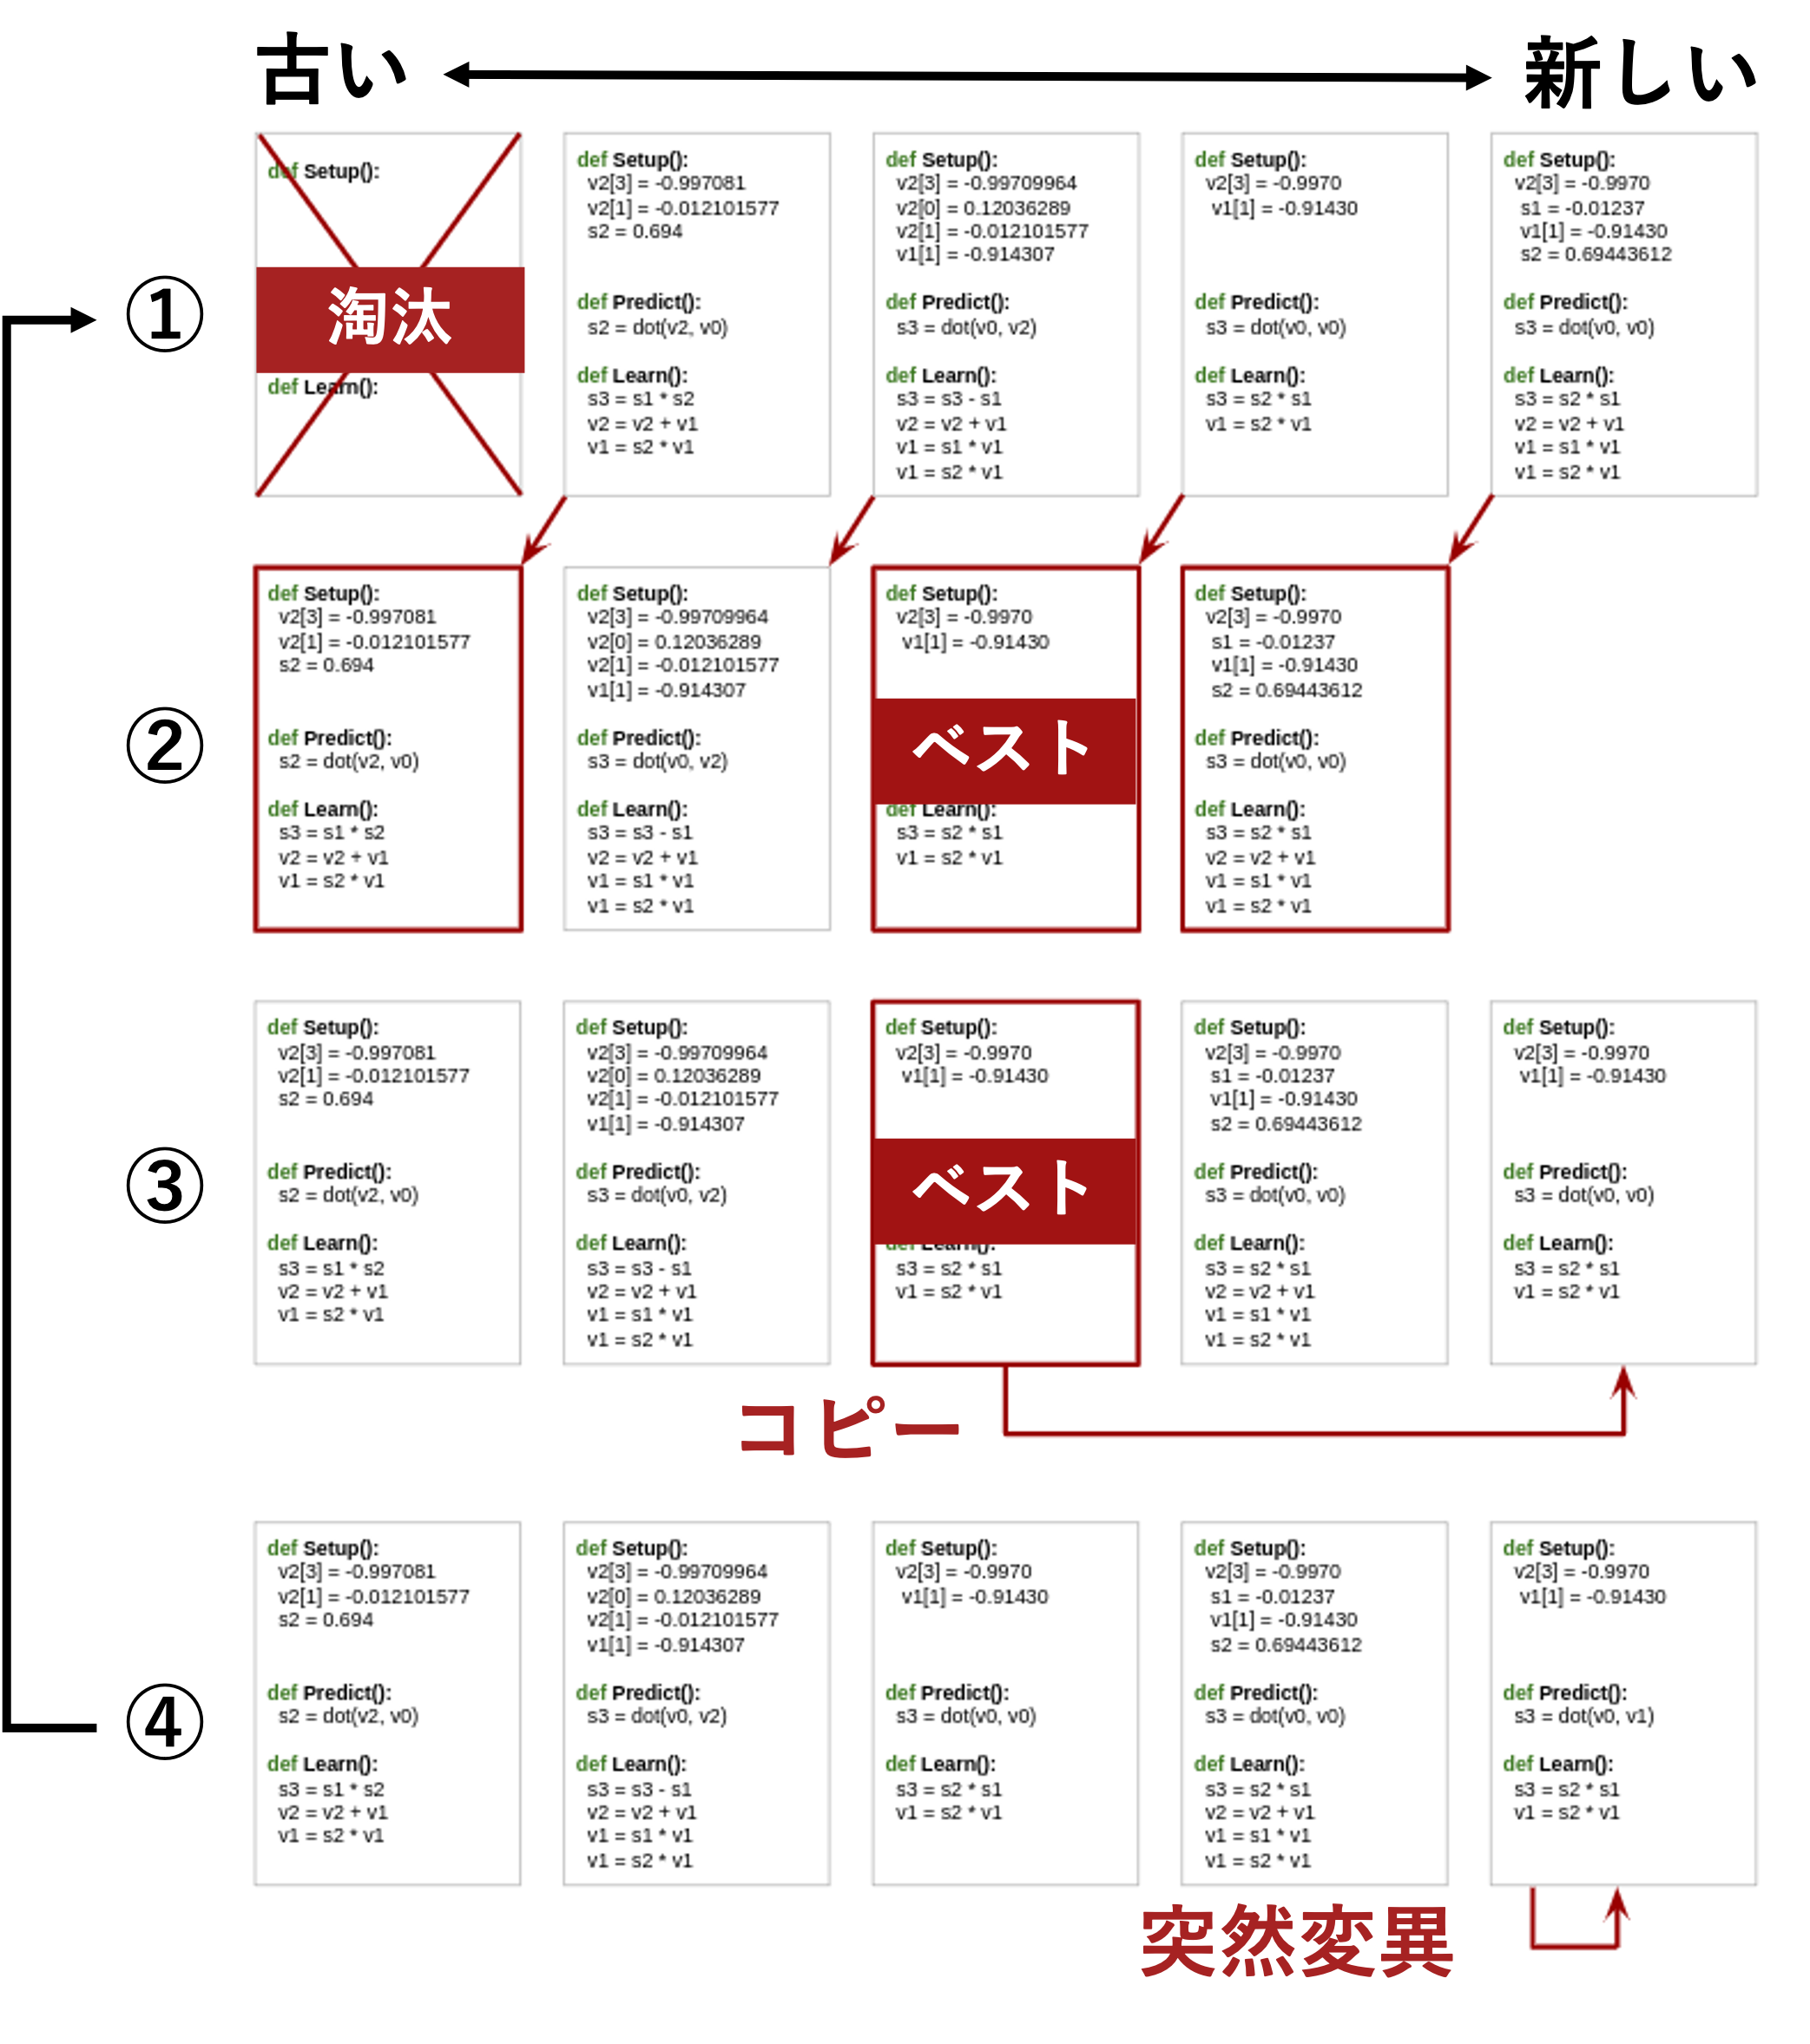
\includegraphics[width=7cm]{re.png}
  \caption{RE-AutoML-Zero\cite{automl_zero}の世代交代モデル}
  \label{fig:regularized_evolution}
\end{figure}

Estebanらが提案したRE-AutoML-Zeroでは, $N_\mathrm{pop}$個のアルゴリズムをランダムに初期集団として生成した後に, Fig.\ref{fig:regularized_evolution}のSTEP1からSTEP4に示したRegularized Evolution (RE) を繰り返し行うことで, 最適なアルゴリズムの探索を行う. REでは, STEP1で最も古い個体を削除した後に, STEP2でトーナメント選択を行う. その後, STEP3でトーナメント選択によって選ばれた個体をコピーし, STEP4で一定確率$p_\mathrm{mutate}$で突然変異を行う. 集団サイズ$N_\mathrm{pop}$, トーナメントサイズ$K$, 突然変異確率$p_\mathrm{mutate}$はユーザパラメータである.

既存手法は, 次の3つの突然変異の手法を用いて子個体を生成する. (1) ランダムに命令を追加または削除する突然変異, (2) 関数のいずれかの命令列全体をランダムに書き換える突然変異, (3) ある命令の入力, 出力, 即値をランダムに変更する突然変異である.

\section{既存手法の問題点}\label{sec:existing_problem}

Estebanらが提案したRE-AutoML-Zeroには, 探索空間の冗長性に関する問題, 良質な構造を子に継承できない問題, 集団の多様維持に関する問題が存在し, 探索が非効率的になっていると考えられる. 以下で, それぞれの問題点について詳しく説明する.

\subsection{探索空間の冗長性に関する問題}\label{subsec:existing_problem:space}

既存手法の探索空間は探索空間が冗長であり, 無意味な評価が多く発生し, 探索効率を低下していると考えられる. 既存手法の冗長性には, 変数名や命令の実行順の違いによる冗長性と非妥当なアルゴリズムによる冗長性の2つが存在する.

変数名や命令の実行順の違いによる冗長性は, Algorithm.\ref{algorithm:algorithm_example}を例に挙げて説明する. Algorithm.\ref{algorithm:algorithm_example}において, $s6$という変数が$s8$に変わったり, 12行目と13行目が入れ替わっても実行結果は同じである. 既存手法では, 実行結果に違いがなく, 変数名や命令の実行順が異なるアルゴリズムを同一視することができず,  探索空間が冗長になっている.

非妥当なアルゴリズムによる冗長性は, 任意の機械学習アルゴリズムにおいて満たすべき条件を満たさないアルゴリズムが探索空間に含まれていることに起因する. 例えば, 正解ラベルや入力ベクトルを全く利用しないアルゴリズム, 代入しても利用されない変数が存在するアルゴリズムなどがその例である. しかし, 既存手法ではこれらの条件を考慮せず, 全てのアルゴリズムを探索しているため, 探索空間に冗長になっている.


\noindent
これらの条件は, 機械学習タスクを高い適合度で解くために, タスクの種類によらず普遍的に必要不可欠な性質であるため, 非妥当なアルゴリズムを探索することは非効率的であると考えられる.

\subsection{良質な構造を子に継承できない問題}\label{subsec:existing_problem:mutation}

既存手法の突然変異は, 親個体が妥当なアルゴリズムであったとしても, 非妥当なアルゴリズムに変化してしまう. 実際, 予備実験の結果により, 妥当な線形回帰アルゴリズムを突然変異させると, 98\%以上の確率で妥当ではないアルゴリズムに変化することが確かめられている.

また, 既存手法では突然変異(2)の関数全体をランダムに変更する破壊的な変化が高頻度で発生するため, 関数中の良質な部分命令列が存在していたとしても, 子個体にその良質な部分命令列が継承ができなくなってしまう可能性が高いと考えられる. 故に, 既存手法の子個体生成方法では, 関数を逐次改善することが難しいと考えられる.

\subsection{集団の多様性維持に関する問題}\label{subsec:existing_problem:diversity}

既存手法は, 集団の多様性が維持しにくく, 局所最適解に陥りやすい問題が存在すると考えられる. 既存手法の世代交代モデルであるREは, 佐藤らの論文\cite{mgg}の考察を踏まえると, 無条件で元の集団の個体が淘汰されている点, 複製選択で強い選択圧が掛かるトーナメント選択が用いられている点, 生存選択で選ばれる個体が淘汰される個体と無関係である点で集団の多様性を失いやすいと考えられる. また, 既存手法では同等の個体や類似個体が考慮されておらず, 希少な構造を持つ個体が他の数の多い個体によって淘汰される可能性が高いと考えられる. これにより, 有望な個体が早期に淘汰され, 局所最適解に収束する問題が生じると考えられる.

\section{提案手法} \label{sec:proposed_method}

提案手法では, 既存手法の問題点として挙げた探索空間の冗長性, 個体の良質な構造を子に継承できない問題, 集団の多様性維持に関する問題に対処した手法を提案する. RE-AutoML-Zeroの人間の事前知識や介入を最小限にできる利点は残しつつ, 探索効率を向上させることを目指す. 提案手法では, グラフ構造を用いてアルゴリズムを表現する手法(アルゴリズムグラフ)とその突然変異を導入することで, 探索空間の冗長性の問題と良質な構造を子に継承できない問題に対処する. また, 集団の多様性維持に関する問題に対処するために, Minimal Generation Gap (MGG) \cite{mgg}による世代交代モデル, 集団内の同一個体の重複排除, および希少度に基づく生存選択を導入する.

\subsection{アルゴリズムグラフ}

\begin{figure}
  \centering
  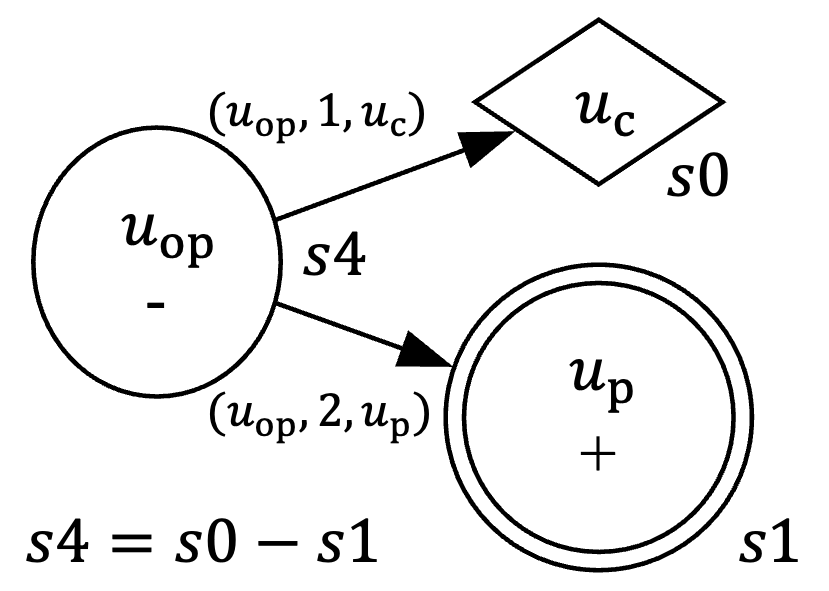
\includegraphics[width=4cm]{op_node.png}
  \caption{Algorithm.\ref{algorithm:algorithm_example}における9行目の命令$s4 = s0 - s1$に対応するAGの命令ノード}
  \label{fig:op_node}
\end{figure}

\begin{figure}
  \centering
  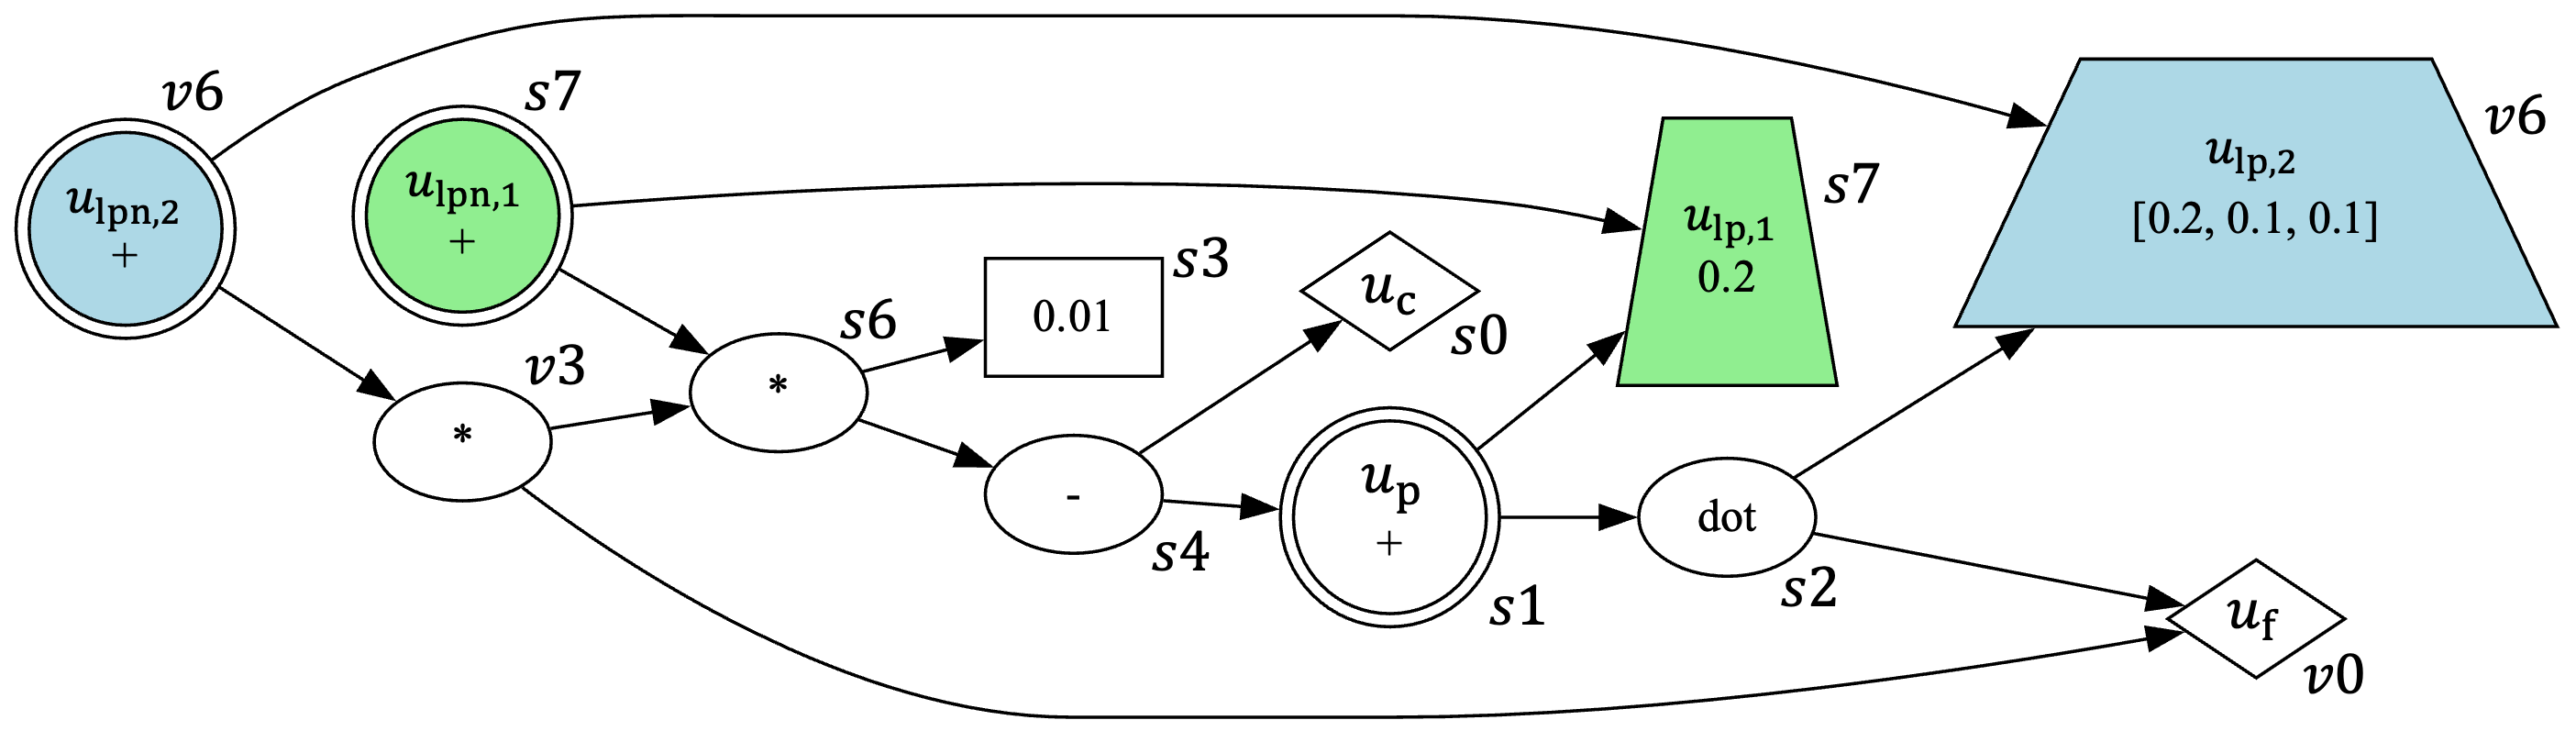
\includegraphics[width=7cm]{affine.png}
  \caption{アフィン回帰と解釈可能なアルゴリズムAlgorithm.\ref{algorithm:algorithm_example}のAG}
  \label{fig:ag_algorithm_example}
\end{figure}

本論文では, アルゴリズムグラフを非巡回順序付き有向グラフ$G = (U, E)$として定式化する. ここで, $U$はノードの集合, $E \subset U \times \mathbb{N} \times U$は順序エッジの集合である. 順序エッジ$(u_1, n, u_2)$は通常の有向グラフのエッジとは異なり, 始点$u_1$と終点$u_2$の他に, $u_1$の何番目のエッジであるかを表す順序値$n \in \mathbb{N}$を持つ.

アルゴリズムグラフ$G = (U, E)$のノード集合$U$に属する各ノードには, 以下の種類が存在する.

\begin{description}
  \item[定数ノード] \ \\ 定数値を表すノードでスカラー, ベクトル, 行列のいずれかの定数値が格納されている.
  \item[入力ベクトルノード: $u_\mathrm{f}$] \ \\ 学習データや検証データの入力ベクトルを代入するノード. 既存手法のアルゴリズムの表現における$v0$に対応する.
  \item[正解ラベルノード: $u_\mathrm{c}$] \ \\ 学習データの正解ラベルを代入するノード. 既存手法のアルゴリズムの表現における$s0$に対応する.
  \item[LPノード: $u_{\mathrm{lp},i}$] \ \\ 学習時に逐次更新される学習パラメータ (Learning Parameter, LP) を表すノード. 学習時の最初のステップでは, 当該学習パラメータの初期値が格納されており, それ以降のステップでは, 1ステップ前で更新された値が格納されている. 一般に複数存在するため, 順序をつけて$u_{\mathrm{lp},i}$と表す.
  \item[命令ノード] \ \\ 命令セット内の命令が割り当てられたノード. 命令の入力に対応するノードを子ノードとして持ち, 命令の出力値が格納されている. $n$番目の子ノードが第$n$引数に対応する. また, 出力の利用用途が特殊な命令ノードとして, 以下の予測ノードとNLPノードが存在する.
  \item[予測ノード: $u_{p}$] \ \\ 出力が予測ラベルとして利用される特殊な命令ノード. 既存手法のアルゴリズムの表現における$s1$に対応する. また, 予測に正解ラベルを利用することはできないため, 予測ノードの子孫ノードに正解ラベルノードを含めることはできない.
  \item[NLPノード: $u_{\mathrm{nlp},i}$] \ \\ 出力が次のステップの特定の学習パラメータ (Next Learning Parameter, NLP) の値として利用される特殊な命令ノード. NLPノードは, $U$内にLPノードと同様の個数存在し, NLPノードとLPノードは1対1で対応するため, 添え字を対応させて$u_{\mathrm{nlp},i}$と表す.
\end{description}
\noindent
各ノードにはスカラー型, ベクトル型, 行列型のいずれかが割り当てられており, 命令ノードの子ノードを割り当てる際は, 命令の入力の型の整合性が保たれる必要がある.

AGにおける1つの命令ノードとそのノードを始点とするエッジは, 第\ref{subsec:existing_problem:algorithm_exp}節で述べた既存手法のアルゴリズムの表現における1行と対応する. 例えば, Fig.\ref{fig:op_node}に示した命令ノード$u_\mathrm{op} \in U$と2つのエッジ$(u_\mathrm{op}, 1, u_\mathrm{c})$と$(u_\mathrm{op}, 2, u_\mathrm{p})$は, Algorithm.\ref{algorithm:algorithm_example}の9行目の命令$s4 = s0 - s1$と対応している.

アフィン回帰と解釈可能なアルゴリズムAlgorithm.\ref{algorithm:algorithm_example}のAGをFig.\ref{fig:ag_algorithm_example}に示す. 図において, 命令ノードは円形, 定数ノードは四角形, データノードはひし形, LPノードは台形で表現されている. 特殊な命令ノードである予測ノードとNLPノードは二重丸で示した. また, 対応関係にあるLPノードとNLPノードは同じ色で着色した. 命令ノードには, 割り当てられている命令の演算子, 定数ノードには代入されている定数値, LPノードには学習パラメータの初期値が記載されている. 子ノードを持つノードの場合は, 図の上部にある子ノードを順序値が小さいものとする. また, アルゴリズムグラフでは不要ではあるが, Algorithm.\ref{algorithm:algorithm_example}との対応関係を明確にするために, 各ノードには代入先の変数名を記載している.

\subsection{妥当なアルゴリズムグラフ}
また, 提案手法では非妥当なアルゴリズムが探索対象とならないように, 以下に示す妥当なアルゴリズムの条件を満たす妥当なアルゴリズムグラフ (Valid Algorithm Graph, VAG) のみを探索対象とする.
\begin{enumerate}
  \item Learn関数で逐次更新される全ての学習パラメータが以下の条件を満たすこと.
  \begin{enumerate}
    \item 1ステップ前の自分自身の値に依存して更新されていること.
    \item Predict関数で利用されている場合は, 正解ラベル$s0$に依存して更新されていること.
    \item Predict関数で利用されている場合は, 予測ラベル$s1$に依存して更新されていること.
  \end{enumerate}
  \item Predict関数で予測ラベル$s1$の算出に, 以下が利用されていること.
  \begin{enumerate}
    \item 入力ベクトル$v0$
    \item 1つ以上のLearn関数で逐次更新される学習パラメータ
  \end{enumerate}
  \item 全ての変数が最終的に予測ラベル$s1$の算出に寄与すること.
\end{enumerate}
\noindent
提案手法ではアルゴリズムをグラフ構造で表現しているため, 妥当なアルゴリズムの条件が成立するか否かの判定が容易である. これにより, 非妥当なアルゴリズムが探索空間に含まれることを効果的に防ぐことができる.

\subsection{初期個体の生成}
提案手法では, VAGのみを探索対象とするために, 予測ノードを起点として, 妥当なアルゴリズムの条件を反映させながら, グラフを段階的に構築していくことでVAGの生成を行う. はじめに, 予測ノードとその子孫ノードに規定の個数になるまで命令ノードを追加する. その後, 予測ノードに必要な依存関係を追加した上で, 空いているはノードにLPノードや定数ノードを追加する.  その後, LPノードに対応するNLPノードとその子孫ノードに規定の個数になるまで命令ノードを追加する. そして、最後にNLPノードに必要な依存関係の追加を行い, VAGが生成される。

\subsection{子個体の生成}

\begin{figure}
  \centering
  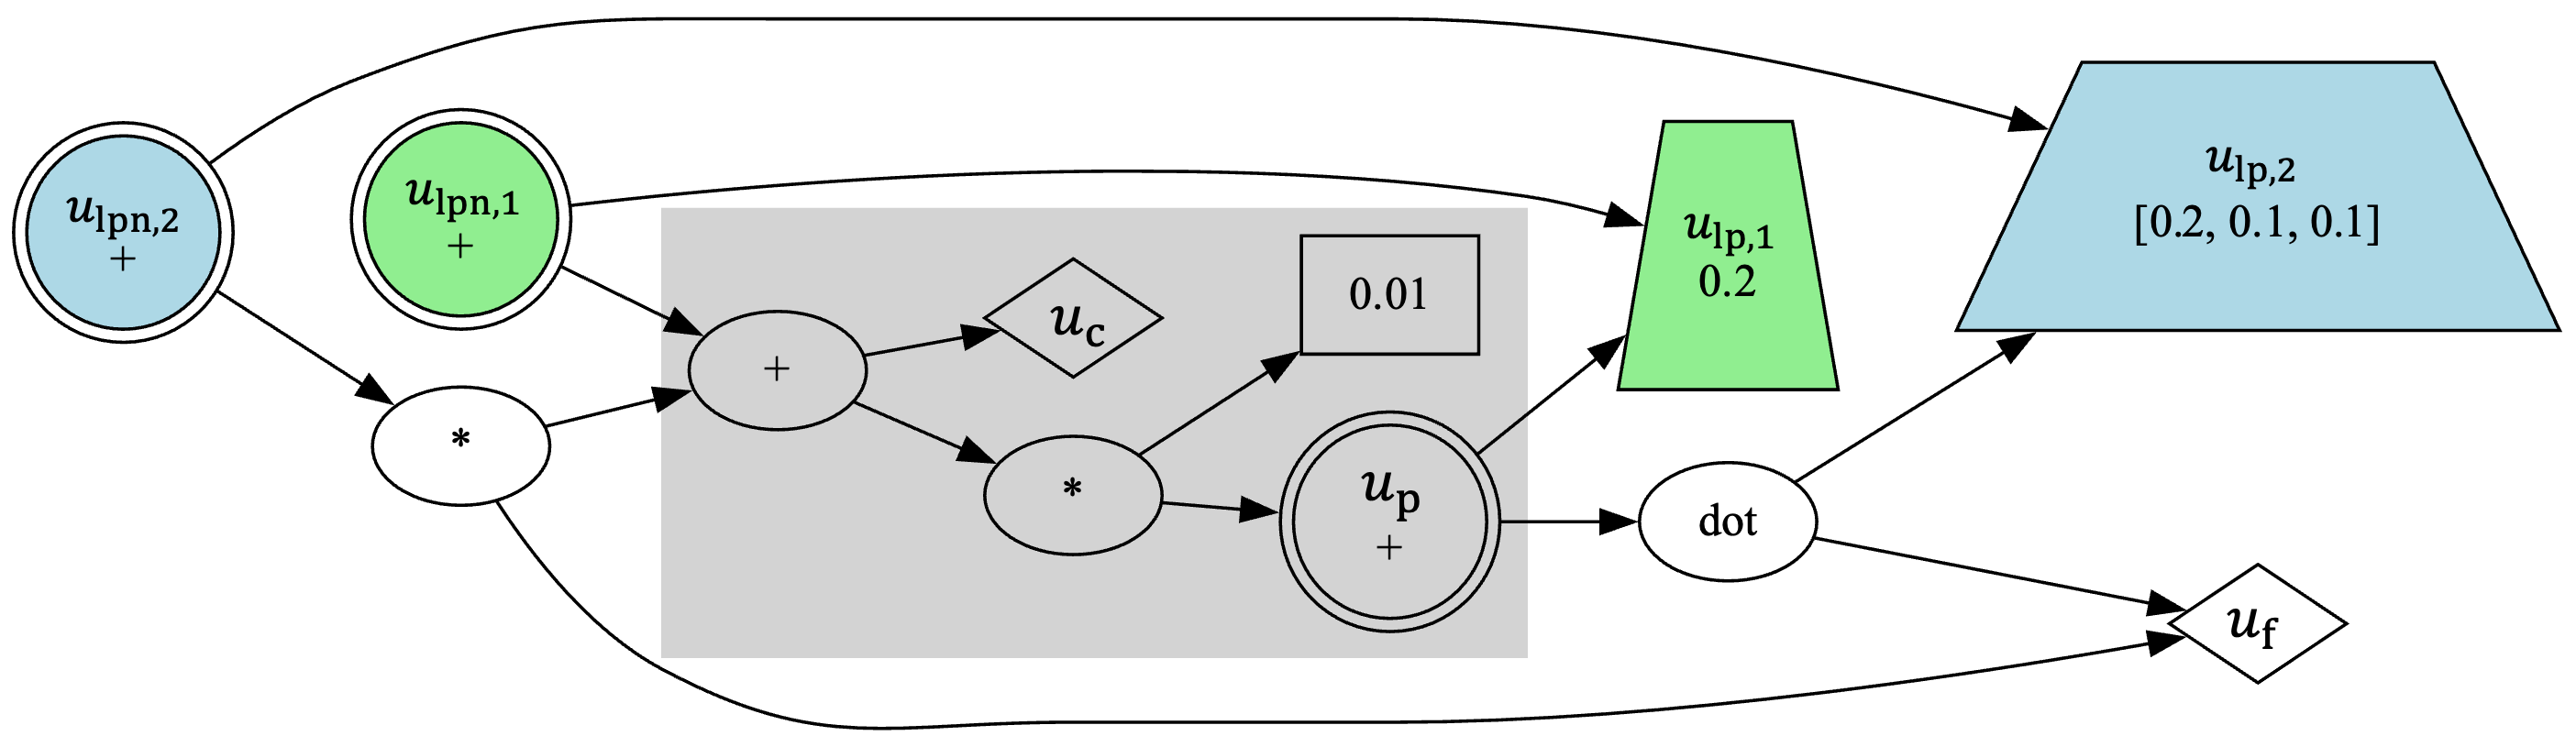
\includegraphics[width=7cm]{subgraph.png}
  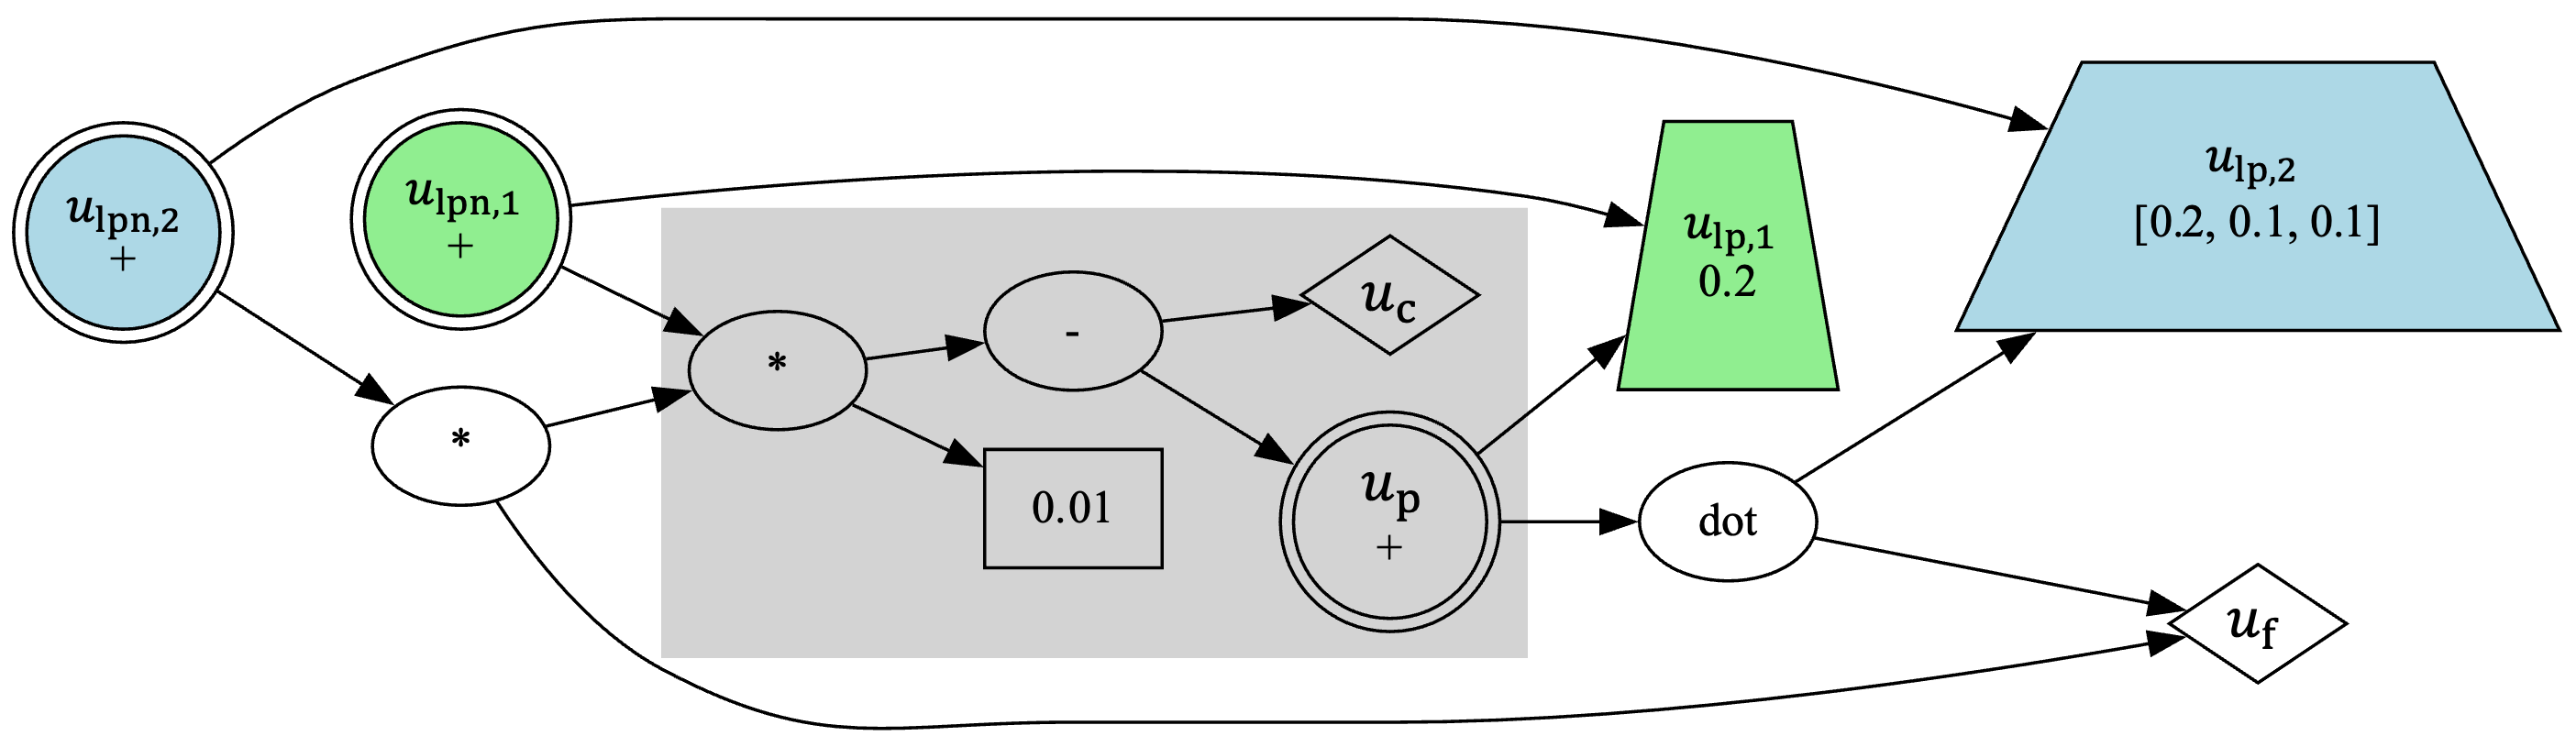
\includegraphics[width=7cm]{mutated_subgraph.png}
  \caption{部分グラフの再構築の突然変異の前後のVAGの様子}
  \label{fig:proposed:mutation:subgraph}
\end{figure}

提案手法では, 子個体に良質な構造を継承できるように, 非妥当なアルゴリズムに変わる突然変異を完全に発生しないようにした上で, グラフ構造を用いた突然変異を導入する. 具体的には, 突然変異後がVAGではない場合は, 再度突然変異を行う. また, 以下の8つのグラフ構造を用いた突然変異を導入し, 既存手法の子個体に良質な構造を継承できない問題に対処する. (1) 定数ノードの値の変更, (2) LPノードの初期値の変更, (3) 定数ノードを接続に置き換え, (4) 接続を定数ノードに置き換え, (5) 接続関係の変更, (6) 部分グラフの再構築, (7) NLPノードをルートとする部分グラフの再構築, (8) 予測ノードをルートする部分グラフの再構築. 突然変異を行う際には, ぞれぞれ所与の選択確率に従って, これらの突然変異操作のいずれかを適用する.

ここでは, 既存手法の問題点を解決する上で最も重要な(6)の部分グラフの再構築の突然変異について, Fig.\ref{fig:proposed:mutation:subgraph}のVAGを例にあげて説明する. 図において, 灰色で示した領域が変更対象となる部分木である. 部分木の突然変異では, 突然変異前後において, ルートノードの型と葉ノードは変化させず, ルートノードの命令の種類や中間ノードの命令とそのエッジを変更する. 部分グラフの再構築による突然変異は, 関数内の特定変数の計算に必要な部分命令列の変更に対応する. 既存手法では関数全体を書き換える突然変異が高頻度で発生し, 良質な部分命令列が破壊的に変更されていた. 一方, 提案手法における部分グラフの再構築は, 関数内の特定変数の計算に必要な部分のみを変更するため, 関数内の良質な部分命令列を維持した突然変異が可能となると考えられる.

\subsection{集団の多様性維持}

\begin{figure}[tbp]
  \centering
  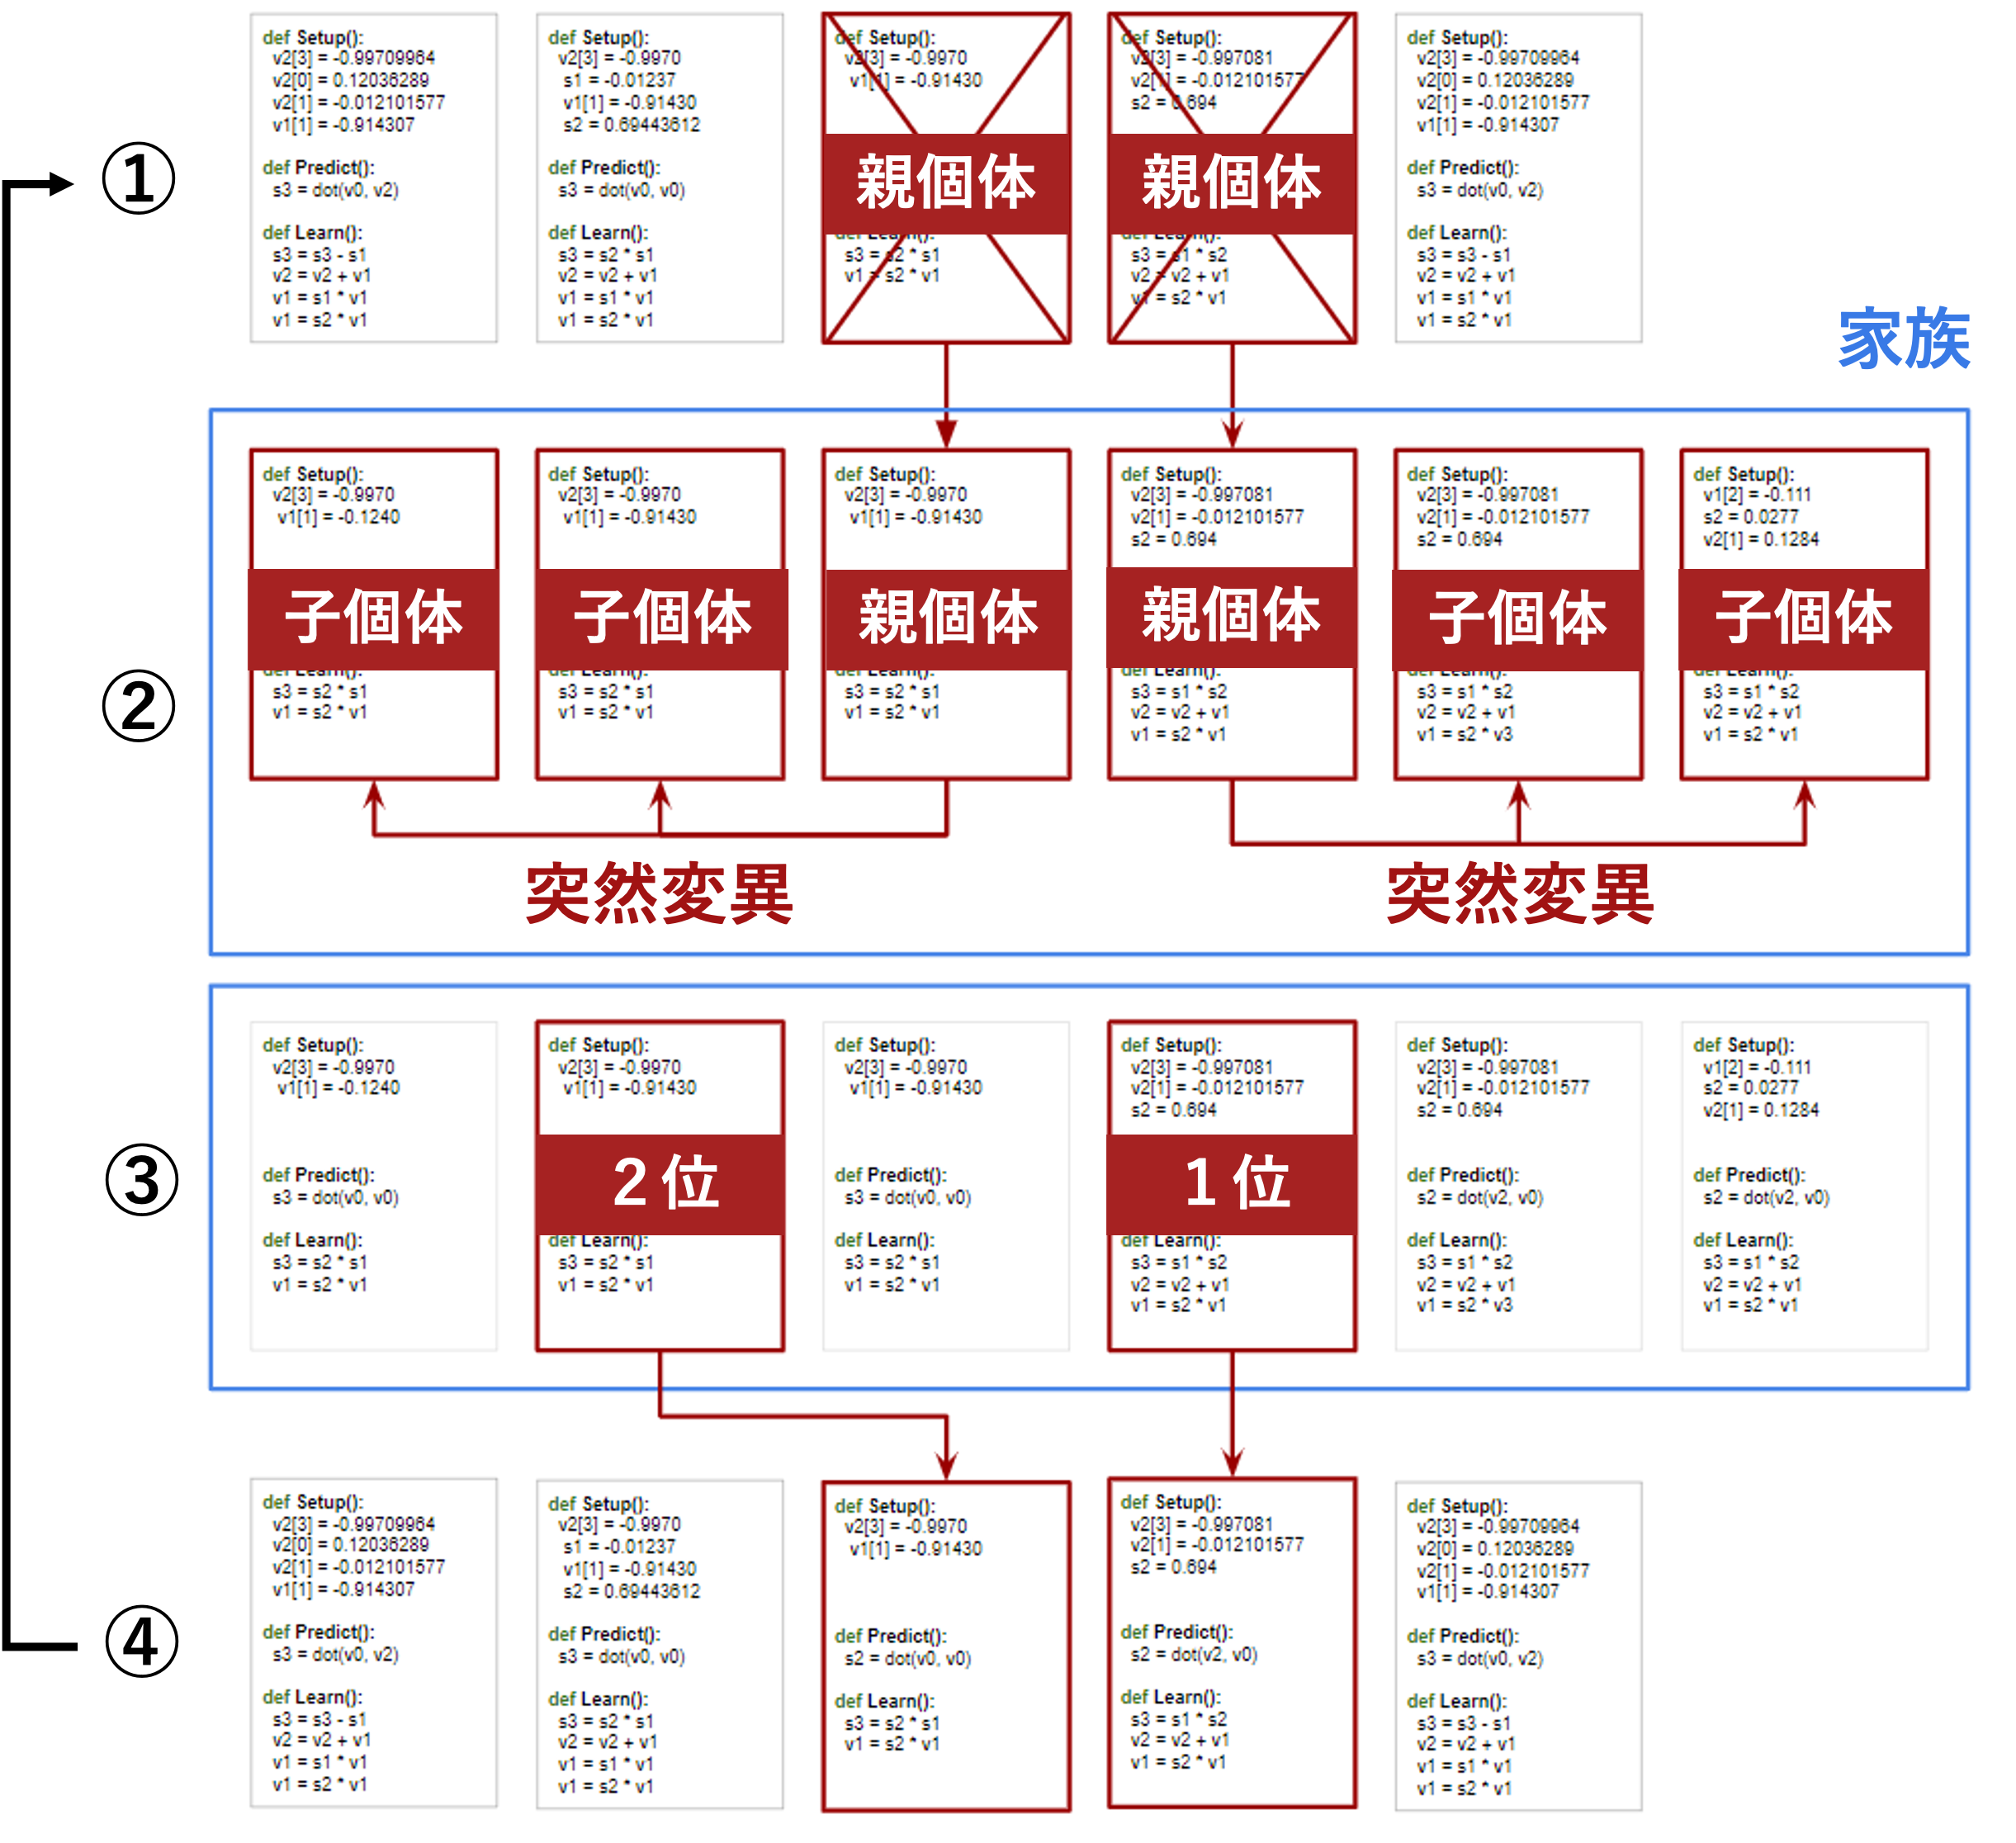
\includegraphics[width=7cm]{./mgg.png}
  \caption{MGGによる世代交代の流れ}
  \label{fig:mgg}
\end{figure}

提案手法では, 集団の多様性を維持しやすくするため, RE-AutoML-Zeroと同様の方法で初期集団を生成した後に, Fig.\ref{fig:mgg}に示したMGGによる世代交代を繰り返し行う. 各世代交代では, STEP1で無作為に2つのアルゴリズム$p_a$, $p_b$を親個体として取り出し, STEP2で$p_a$を突然変異させた個体を$N_\mathrm{children} / 2$個, $p_b$を突然変異させた個体を$N_\mathrm{children} / 2$個つくり, 合計で$N_\mathrm{children}$個の子個体を生成する. その後のSTEP3,4では, 生成した$N_\mathrm{children}$個の子個体と親個体$p_a$, $p_b$を合わせた家族に対して生存選択で2つ個体を選択して集団に戻す. 集団サイズ$N_\mathrm{pop}$, 子個体生成数$N_\mathrm{children}$はユーザパラメータである.

世代交代モデルをMGGに置き換えることで, 第\ref{subsec:existing_problem:diversity}節で述べた3つの集団の多様性を低下させる要因に対処できると考えられる. MGGでは, Fig.\ref{fig:mgg}のSTEP1で淘汰される候補となった親個体も, Fig.\ref{fig:mgg}のSTEP3, 4の生存選択で集団に戻される可能性があるため, 集団内の個体が無条件で淘汰されることはない. また, Fig.\ref{fig:mgg}のSTEP1で無作為に複製選択するため, トーナメント選択のような強い選択圧がかかりにくいと考えられる. 加えて, STEP3, 4における生存選択で選ばれる個体が, 淘汰される候補である親個体の家族に限定されているため, 淘汰される個体と無関係な個体が次世代に引き継がれることが少ない.

さらに, 提案手法では同一の個体や類似の個体が集団内に増えることを抑制するために, 集団内の同一個体の重複排除と希少度を考慮した生存選択を行う. 重複排除は, 集団内の個体の重複を検知し, 重複している個体を削除することで, 集団内の多様性を維持することができる. 希少度を考慮した生存選択では, 定数や学習パラメータの値のみが異なるアルゴリズムを類似個体と判定し, 集団内の個体の希少度を計算し, 希少度が高い個体を優先的に選択する. これにより, 集団内の多様性を維持し, 局所最適解に収束する可能性を低減することができると考えられる.

\section{実験} \label{sec:exp}

\subsection{目的}\label{subsec:exp:purpose}

本実験の目的は, 回帰アルゴリズムや分類アルゴリズムの探索問題をローカルPCの少ない計算リソース上で実行し, 提案手法と既存手法の探索性能を比較をすることである. 既存手法であるEstebanらの手法RE-AutoML-Zero\cite{automl_zero}に比べて, 提案手法のMGG-AutoML-Zero+VAGの方が, 所与の評価回数で高い適合度のアルゴリズムが得られることを確認する.

\subsection{実験設定}\label{subsec:exp:setting}
本実験では, 回帰問題と分類問題それぞれで, 線形, アフィン, 非線形の特性を持つ問題を用いる. それぞれの問題に対して, ノイズがない場合とノイズが正規分布$N(0,0.1)$に従う場合の2種類の問題を用意し, 合計12種類問題で実験を行う.

\subsection{評価基準}\label{subsec:exp:eval}

本実験では, それぞれの問題設定で乱数を変えて10試行の実験を行い, 所与の評価回数までに発見されたアルゴリズムの適合度の平均値を評価基準とする. 適合度は回帰問題の場合であれば全てのタスクの検証データに対して完全に誤差なしで回帰できた場合に1, 分類問題であれば全てのタスクの検証データを正しく分類できた場合に1となる. また, 各実験における打ち切り適合度は0.999, 打ち切り評価回数は線形回帰/分類の問題では20,000回, アフィン回帰/分類の問題では2,000,000回, 非線形回帰/分類の問題では20,000,000回とした.

\subsection{実験結果}\label{subsec:exp:result}
実験の結果をTable.\ref{table:exp:result}に示す. 実験結果より, 全ての問題設定において, 提案手法は既存手法よりも高い適合度のアルゴリズムの発見に成功していることが確認できる.

\begin{table*}[tbp]
  \caption{既存手法と提案手法の実験結果}
  \label{table:exp:result}
  \centering
  \begin{tabular}{|c|c|c|c|}
    \hline
    \multicolumn{2}{|c|}{問題} & 既存手法 & 提案手法 \\
    \hline
    \multirow{2}{*}{線形回帰}
    & ノイズなし  & $ 0.399 \pm 0.032$ & $\bm{1.000 \pm 0.000}$  \\
    & ノイズあり  & $ 0.400 \pm 0.036$ & $\bm{0.931 \pm 0.006}$  \\
    \multirow{2}{*}{線形分類}
    & ノイズなし  & $ 0.978 \pm 0.009$ & $\bm{0.980 \pm 0.009}$  \\
    & ノイズあり  & $ 0.973 \pm 0.008$ & $\bm{0.972 \pm 0.005}$  \\
    \multirow{2}{*}{アフィン回帰}
    & ノイズなし  & $ 0.586 \pm 0.256$ & $\bm{1.000 \pm 0.000}$  \\
    & ノイズあり  & $ 0.431 \pm 0.159$ & $\bm{0.936 \pm 0.002}$  \\
    \multirow{2}{*}{アフィン分類}
    & ノイズなし  & $ 0.863 \pm 0.079$ & $\bm{0.983 \pm 0.003}$  \\
    & ノイズあり  & $ 0.917 \pm 0.056$ & $\bm{0.977 \pm 0.004}$  \\
    \multirow{2}{*}{非線形回帰}
    & ノイズなし  & $ 0.360 \pm 0.059$ & $\bm{0.536 \pm 0.098}$  \\
    & ノイズあり  & $ 0.364 \pm 0.058$ & $\bm{0.519 \pm 0.127}$  \\
    \multirow{2}{*}{非線形分類}
    & ノイズなし  & $ 0.876 \pm 0.447$ & $\bm{0.961 \pm 0.011}$  \\
    & ノイズあり  & $ 0.854 \pm 0.029$ & $\bm{0.918 \pm 0.016}$  \\
    \hline
  \end{tabular}
\end{table*}

\section{考察} \label{sec:discussion}

\subsection{探索効率}
\begin{figure}
  \centering
  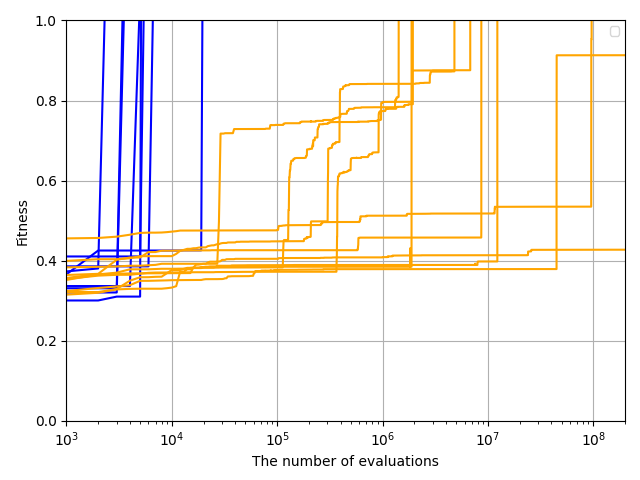
\includegraphics[width=7cm]{liner_regression.png}
  \caption{線形回帰問題における最適解発見まで評価値の推移(青:提案手法, 橙:既存手法)}
  \label{fig:discussion:efficiency}
\end{figure}

本節では, 提案手法の探索効率がどの程度向上しているかを定量的に評価するために, 第\ref{sec:exp}章の線形回帰の問題設定で, 適合度が1.00になる最適解の発見までにかかる評価回数を比較する実験を行った. 乱数を変えて, 10試行行った時の評価値の改善推移をFig.\ref{fig:discussion:efficiency}に示す. 実験結果より, 提案手法は既存手法に比べて, 少ない評価回数で最適解を発見できていることがわかる. 定量的には, 既存手法が平均5,399,857回の評価回数で最適解を発見したのに対し, 提案手法は平均5,270回の評価回数で最適解を発見しており, 必要な評価回数はおよそ1/1000倍になっていることがわかった.


\subsection{発見されたアルゴリズム}

第\ref{sec:exp}章の実験で発見された非線形回帰アルゴリズムをAlgorithm.\ref{algorithm:optimum}に示す. このアルゴリズムを解釈すると, 活性化関数がReLUの1層のニューラルネットワークと類似したアルゴリズムであることとがわかる. 特に, Learn関数では, ReLU関数の導関数である$\mathrm{heaviside}$関数で勾配の計算をした上で, ニューラルネットワークの重みに対する勾配降下法を適用していると考えられる.

\begin{algorithm}[tb]
  \caption{提案手法で発見された非線形回帰のアルゴリズム (Setup関数は省略)}
  \label{algorithm:optimum}
  \begin{algorithmic}[1]
    \Function{Predict}{}
    \State $v8 = \mathrm{dot}(m0, v0)$
    \State $v10 = \mathrm{maximum}(v8, v1)$
    \State $s1 = \mathrm{dot}(v9, v10)$
    \EndFunction
    \Function{Learn}{}
    \State $s2 = s0 - s1$
    \State $v5 = s2 * v9$
    \State $v7 = \mathrm{heaviside}(v8, 1.0)$
    \State $v6 = s3 * v7$
    \State $v3 = v5 * v6$
    \State $v2 = s2 * v4$
    \State $m1 = \mathrm{outer}(v3, v0)$
    \State $v1 = v1 + v2$
    \State $m0 = m0 + m1$
    \EndFunction
  \end{algorithmic}
\end{algorithm}


\section{おわりに}
\subsection{まとめ}
本論文では, Estebanらが提案したRE-AutoML-Zeroの探索効率に対する問題点を指摘した上で, その問題点に対処した手法の提案を行った. 提案手法では, グラフ構造を用いてアルゴリズムを表現する手法(アルゴリズムグラフ)とその突然変異を導入することで, 探索空間の冗長性の問題と良質な構造を子に継承できない問題に対処した. また, 集団の多様性維持に関する問題に対処するために, Minimal Generation Gap (MGG) \cite{mgg}による世代交代モデル, 集団内の同一個体の重複排除, および希少度に基づく生存選択を導入した.

その結果, 回帰問題や分類問題の主要なベンチマークにおいて, 提案手法は既存手法よりも高い適合度のアルゴリズムの発見に成功し, 線形回帰アルゴリズム問題では, 最適解発見までに必要な評価回数が1/1000になることが確かめられた.

\subsection{今後の課題}
本研究の今後の課題として, ハイパーパラメータのチューニング, 高度な問題設定による大規模実験の実施, VAGの交差の実現の3つが挙げられる. 各突然変異の選択確率等のハイパーパラメータは, 探索の進捗に合わせて動的に設定することで, 探索効率の改善が期待できる. また, 本論文の実験では, 限られた命令セットで機械学習の問題設定の中でも比較的簡単な問題を扱って, 探索性能の確認を行った. その結果, 提案手法は既存手法の1000倍以上の性能を持つことが確認できたので, より大規模な問題に挑戦していきたい. また, 現状は1つのVAGに対する突然変異のみで, 複数の親個体の構造を継承することができない, そのため, VAGの交叉手法を開発し, 複数の親個体の構造を継承できるようにし, より効率的に探索を行うことが課題である.

\bibliographystyle{jplain}
\bibliography{ref}

\end{document}
